\chapter{Continuous Immigrant Local Inhibition and Synthetic Control Regimes}
\label{ch:local-inhibition}
\section{Study overview}

The registered continuous local-inhibition (LI) procedure selects exactly zero inhibition strength in all three previously inspected California test windows. Across the same 315 targets used in the preceding comparisons, LI is a numerical tie with matched Omori continuous (OC); its raw pooled positive difference is only 1.884928e-10 total nats and is not a predictive gain. The inverse-power ETAS benchmark (EP) remains better jointly in every window, mainly through conditional location. In the historical initial control study, all eight fixed-seed controls are retained: LI loses to OC on both uniform-null, both smooth-null and both narrow/short-inhibition datasets, and wins on both broad/long-inhibition datasets. Two seeds per regime cannot estimate power or a false-positive rate, and the narrow/short losses prevent a claim that this procedure would reliably detect inhibition when present. At zero inhibition, range and memory are unidentified. These results concern a frozen statistical extension that attenuates only the immigrant component at recorded coordinates; they do not establish absence of physical inhibition, causal mechanisms, significance or global optimization.

\section{Key question and review status}

Does spatially local, temporary attenuation improve retrospective prediction beyond the matched OC procedure, and does the resulting procedure compete with EP? The question follows the positive continuous-location ablation in Chapter~\ref{ch:nz-spatial} and the more qualified external, benchmark and diagnostic findings in Chapter~\ref{ch:external}. It requires an actual likelihood with full exposure, a frozen fitting rule, matched references, retained negative controls and complete accounting. A term described as inhibition is not evidence that a physical stress-depletion mechanism has been identified.

The historical source is the accepted initial local-inhibition completion, including its selected-state diagnostics, aggregate checker and preservation audits. Its results remain identified separately from the expanded controls in Section~\ref{sec:s04-expanded}, which report new numerical follow-up. The historical source authorities remain unchanged. It activates no live forecast. Underlying independent computational review is distinct from external academic inspection; the latter remains pending for this package.

\section{Recorded-event design and comparator definitions}

\subsection{Same California history, not a new sample}

The observation law selects preferred California records with reported M $\geq$ 4.0, latitude 32-37 degrees, longitude -121 to -114 degrees and depth -5 to 40 km. The fixed source contains 1,272 unique events: 106 warmup parents in 1981-1985 and 1,166 evaluated records in 1986-2026. The latter comprise 851 initial training targets plus 315 subsequent test targets. Warmup is already included in 1,272; the counts must not be added a second time.

\begingroup\footnotesize\setlength{\tabcolsep}{2pt}\renewcommand{\arraystretch}{1.18}
\begin{longtable}{@{}>{\raggedright\arraybackslash}p{0.1800\textwidth}>{\raggedright\arraybackslash}p{0.1800\textwidth}>{\raggedright\arraybackslash}p{0.1800\textwidth}>{\raggedright\arraybackslash}p{0.1800\textwidth}>{\raggedright\arraybackslash}p{0.1800\textwidth}@{}}
\toprule
{}Fold & Test window, UTC & Training targets & Test targets & Exposure days \\
\midrule\endfirsthead
\toprule
Fold & Test window, UTC & Training targets & Test targets & Exposure days \\
\midrule\endhead
\midrule\multicolumn{5}{r}{\emph{Continued on next page}}\\
\endfoot
\bottomrule\endlastfoot
{}F0 & 2011-2016 & 851 & 79 & 1,826 \\
{}F1 & 2016-2021 & 930 & 167 & 1,827 \\
{}F2 & 2021-2026 & 1,097 & 69 & 1,826 \\
{}Pooled test & 2011-2026 & Overlapping prefixes & 315 & 5,479 \\
\end{longtable}\endgroup

These are the same 315 targets in the California replication, benchmark, conditional diagnostic and concentration studies. Their repeated evaluation is not independent replication. The archive and earlier annual/sequence outcomes had already been inspected. Parameters and nuisance choices use training data, remain frozen in test, and histories update sequentially after each observed timestamp. Only strictly earlier eligible events enter excitation and inhibition; timestamp ties are processed as a batch, with no within-batch self- or mutual influence.

\subsection{The references answer different questions}

OC means Omori temporal triggering with the finite-domain continuous, reference-density-weighted offspring law and smooth immigrant background. EP means a separately fitted Omori ETAS adaptation whose inverse-power radial offspring density is normalized directly against projected area without OC's reference weighting. EP is an excitation model, not a Poisson model. LI-OC is the matched extension comparison. LI-EP compares complete competing procedures with different spatial excitation laws and does not isolate inhibition alone.

For completeness, the other abbreviations in the programme are FC (fixed-scale Mittag-Leffler continuous), FL (its cell-lift counterpart), OL (Omori cell-lift), MC (free common-scale Mittag-Leffler continuous) and N0 (a separately refitted smooth no-trigger procedure). Their primary contrasts are detailed in Chapter~\ref{ch:external}. A constant-Poisson candidate here is a numerical optimization floor, distinct from N0 and EP.

\section{The continuous immigrant-inhibition model}

\subsection{Intensity and attenuation field}

For time t and recorded projected location z in the fixed finite domain D, the model is

\begin{align}
\lambda_{\rm LI}(t,z)&=e^{a+dx_{\mathrm{trend}}(t)}b_{\rm bg}(z)e^{-\eta G(t,z)}+nH_{\rm OC}(t,z),\label{eq:spatial-li-intensity}\\
x_{\mathrm{trend}}(t)&=2t/T_0-1,\qquad T_0=16436\ \text{days},\\
G(t,z)&=\sum_{j:t_j<t}e^{-(t-t_j)/\psi}
\left(1+\frac{\lVert z-z_j\rVert^2}{\ell^2}\right)^{-2}.\label{eq:spatial-li-field}
\end{align}
The observed clock is days since 1981-01-01 00:00:00 UTC.

Here $a$ and $d$ govern immigrant amplitude/trend; $b_{\rm bg}$ is the inherited training-only background density; $n$ scales excitation $H_{\rm OC}$; $\eta$ is nonnegative inhibition strength; $\ell$ is its spatial range in kilometres; and $\psi$ is its memory in days. The observed clock uses the frozen timestamp convention and strict earlier-integer-timestamp parent rule, including tied batches. Synthetic controls have their own day-zero origin and normalization, specified in Section~\ref{sec:li-generating-contract}. The stress mark multiplier is fixed to one: every eligible earlier recorded event contributes to $G$ without magnitude weighting. No latent immigrant/offspring classification is required. Inhibition acts only on the immigrant term. It does not suppress $H_{\rm OC}$, and it is not spatially renormalized. It therefore changes both local density and total immigrant rate. Renormalizing the inhibited density would define a different model.

The unit stress mark is a substantive restriction: at the same lag and separation, an eligible M4 event and an eligible M7.1 event contribute equally to the attenuation field. Their excitation productivity can still differ through $\kappa_j$. This model therefore does not represent magnitude-scaled stress release, a Coulomb stress tensor, or suppression of the full triggered sequence. It tests immigrant attenuation under one restricted statistical law.

More explicitly, the inherited excitation is a sum over all eligible strictly earlier parents:

\begin{align}
H_{\rm OC}(t,z)&=\sum_{j:t_j<t}\kappa_j k_O(t-t_j)s_\sigma(z\mid z_j),\\
k_O(u)&=\frac{(p-1)c^{p-1}}{(u+c)^p},\qquad u>0,\\
s_\sigma(z\mid z_j)&=\frac{b_{\rm ref}(z)(1+\lVert z-z_j\rVert^2/\sigma^2)^{-2}}{Z_j},\label{eq:spatial-normalized-density}\\
Z_j&=\int_D b_{\rm ref}(v)(1+\lVert v-z_j\rVert^2/\sigma^2)^{-2}\,\mathrm dv.
\end{align}

Here $\kappa_j$ is the shared training-calibrated magnitude-productivity weight, with fixed exponent $r=0.7$; $b_{\rm ref}$ is the frozen training-derived reference geography. The background $b_{\rm bg}$ integrates to one on $D$. The temporal kernel integrates to one over all positive lags and each $s_\sigma$ integrates to one on $D$; exposures use the actual finite time window. The training-only smooth background, parent eligibility and inherited excitation nuisance choices follow the matched OC procedure. LI introduces no new background bandwidth or excitation spatial-scale search. The stress radial factor in $G$ itself is not a normalized spatial probability density; it is an attenuation field inside the exponential.

The temporal factor is the normalized Omori--Utsu law \citep{Utsu1995}; the reference-weighted spatial factor is a particular fitted forecasting choice rather than a physical stress law.

At $\eta$ = 0, $\exp[-\eta G]$ equals one everywhere and LI exactly nests OC when shared coordinates agree. All $\ell$ and $\psi$ choices then give the same law. Canonical $\ell$ = 30 km and $\psi$ = 7 days are display conventions at that boundary, not recovered scales. Even a positive procedure score difference at $\eta$ = 0 could arise from refitting shared coordinates through another optimization path; it would not establish active attenuation. The separate approved selected-state diagnostics are therefore essential to the conclusion below.

\subsection{Frozen fitting and selection contract}

The fitted coordinates are $(a,d,n,\log c,p,\eta,\log\ell,\log\psi)$, where $c$ and $p$ parameterize the normalized Omori kernel. The physical bounds are fixed.

\begingroup\small\setlength{\tabcolsep}{2pt}\renewcommand{\arraystretch}{1.18}
\begin{longtable}{@{}>{\raggedright\arraybackslash}p{0.2280\textwidth}>{\raggedright\arraybackslash}p{0.2280\textwidth}>{\raggedright\arraybackslash}p{0.2280\textwidth}>{\raggedright\arraybackslash}p{0.2280\textwidth}@{}}
\toprule
{}Coordinate & Bound & Coordinate & Bound \\
\midrule\endfirsthead
\toprule
Coordinate & Bound & Coordinate & Bound \\
\midrule\endhead
\midrule\multicolumn{4}{r}{\emph{Continued on next page}}\\
\endfoot
\bottomrule\endlastfoot
{}a & [-12, 0] & d & [-2, 2] \\
{}n & [0, 0.98] & c & [0.0001, 20] days \\
{}p & [1.01, 2.5] & $\eta$ & [0, 4] \\
{}$\ell$ & [5, 150] km & $\psi$ & [1/24, 365] days \\
\end{longtable}\endgroup

Each main arm has eight prescribed starts. For LI fits only, shared a,d,n start from the accepted matched OC state. LI start 0 retains OC's c,p and $\eta$ = 0; the other LI starts use the fixed c,p,$\eta$,$\ell$,$\psi$ schedule below. Synthetic OC control fits use a separate frozen initialization rule, not their own subsequently accepted fit: a0 = clip(log(0.6 max(Ntrain,1)/365), -11.5, -0.1), d0 = 0.2 and n0 = 0.35, with eight prescribed c,p rows in synthetic\_\allowbreak{}common/OC\_\allowbreak{}start\_\allowbreak{}fill. The readable protocol subset gives both start schemes, floors, bounds and tolerances in full.

L-BFGS-B has maxiter 200, maxfun 20,000, maxls 200, ftol 1e-10 and gtol 2e-6. Bounded Powell is allowed only after failure of the declared first-method acceptance rule, from the same original start, with maxiter 400, maxfev 5,000, xtol 1e-6 and ftol 1e-10. These limits describe a bounded search, not a global optimization proof.

\begingroup\small\setlength{\tabcolsep}{2pt}\renewcommand{\arraystretch}{1.18}
\begin{longtable}{@{}>{\raggedright\arraybackslash}p{0.2280\textwidth}>{\raggedright\arraybackslash}p{0.2280\textwidth}>{\raggedright\arraybackslash}p{0.2280\textwidth}>{\raggedright\arraybackslash}p{0.2280\textwidth}@{}}
\toprule
{}LI start: c (days), p & $\eta$ & $\ell$ (km) & $\psi$ (days) \\
\midrule\endfirsthead
\toprule
LI start: c (days), p & $\eta$ & $\ell$ (km) & $\psi$ (days) \\
\midrule\endhead
\midrule\multicolumn{4}{r}{\emph{Continued on next page}}\\
\endfoot
\bottomrule\endlastfoot
{}0: accepted OC c,p & 0 & 30 & 7 \\
{}1: 0.0001, 1.1 & 0.1 & 5 & 1/24 \\
{}2: 0.001, 1.3 & 0.3 & 15 & 0.25 \\
{}3: 0.01, 1.1 & 0.7 & 50 & 7 \\
{}4: 0.1, 1.3 & 1.5 & 150 & 30 \\
{}5: 1, 1.7 & 3 & 5 & 365 \\
{}6: 20, 2.5 & 4 & 150 & 1/24 \\
{}7: 0.1, 1.01 & 0.5 & 30 & 365 \\
\end{longtable}\endgroup

Selection minimizes accepted training joint negative log likelihood. Exact ties prefer the OC floor, then the Poisson floor, then start and method ordinals. Held-out score does not select a candidate, method, computational epoch or seed. Candidates within 0.0004 training NLL units of the selected state receive the declared held-out spread check, requiring spread strictly below 0.01 nats per target. This is an admission/sensitivity diagnostic over the stored near-optimal set; it is neither an uncertainty interval nor permission to select the best test forecast.

The readable protocol subset and exact data-free case matrix copy expose the full start schedules, law, observation scope and selection rule; source pins bind their identities. The case matrix retains historical execution-status labels; final accepted completion receipts establish the results status. An earlier methods proposal is contextual, and the structured frozen case matrix is authoritative where it differs.

\subsection{Proper scores and exposure}

Write P for summed event log point intensity, Q for summed event log regional intensity, E for positive full-domain integrated intensity, C = -E for its signed score contribution and M for the common magnitude-mark score. Then

\begin{align}
S_{\rm time}&=Q+C=Q-E,&S_{\rm loc}&=P-Q,\\
S_{\rm joint}&=P+C+M=S_{\rm time}+S_{\rm loc}+M,\\
\Delta P&=P_{\rm LI}-P_R,&\Delta C&=E_R-E_{\rm LI},\\
\Delta S_{\rm joint}&=\Delta P+\Delta C+\Delta M.
\end{align}

All quiet-period and full-domain exposure is retained. Lower exposure can offset a worse event-intensity term; an event-only gain is insufficient. Within each arm, Q uses that arm's spatially integrated ground intensity under the fixed observed history, and all components use its same fitted state. Independently fitted arms can have different parameters. The shared conditional mark law is scored once and cancels in contrasts. Pooled scores sum all three window totals and divide by 315. These are nats of realised predictive log score, not percent accuracy, correlation, a physical effect size or evidence of calibration.

The source-field dictionary distinguishes these narrative symbols from legacy aggregate keys. In particular, LI's raw pooled E field means the point-event logsum difference, not positive exposure; its raw C is the signed exposure contribution. Sequence timing\_\allowbreak{}compensator instead stores signed difference in nonnegative integrated exposure and enters the score negatively. Source keys and scalars remain unchanged.

\section{Observed result: no selected inhibition and a numerical tie}

All three selected LI fits have $\eta$ \textbf{exactly zero}. The procedure selects no active attenuation term in these observed windows. Its joint contrasts against OC are numerical ties under the frozen aggregate sign tolerance of +/-0.0002 total nats (inclusive).

\begingroup\footnotesize\setlength{\tabcolsep}{2pt}\renewcommand{\arraystretch}{1.18}
\begin{longtable}{@{}>{\raggedright\arraybackslash}p{0.1800\textwidth}>{\raggedright\arraybackslash}p{0.1800\textwidth}>{\raggedright\arraybackslash}p{0.1800\textwidth}>{\raggedright\arraybackslash}p{0.1800\textwidth}>{\raggedright\arraybackslash}p{0.1800\textwidth}@{}}
\toprule
{}Window & Targets & LI-OC joint nats/target & Selected $\eta$ & Interpretation \\
\midrule\endfirsthead
\toprule
Window & Targets & LI-OC joint nats/target & Selected $\eta$ & Interpretation \\
\midrule\endhead
\midrule\multicolumn{5}{r}{\emph{Continued on next page}}\\
\endfoot
\bottomrule\endlastfoot
{}F0 & 79 & 0 & 0 & Numerical tie \\
{}F1 & 167 & +1.128699e-12 & 0 & Numerical tie \\
{}F2 & 69 & 0 & 0 & Numerical tie \\
{}Pooled & 315 & +5.983898e-13 & 0 in 3/3 & Numerical tie \\
\end{longtable}\endgroup

The raw pooled difference is +1.88492776942439e-10 total nats. Its tiny positive floating-point sign is retained for arithmetic traceability and is not a forecast improvement. The frozen aggregate sign tolerance concerns numerical comparison, not statistical significance or a fitter admission gate. Exact model nesting and finite arithmetic are separate issues: the selected law has no inhibition, while independently evaluated saved score arithmetic may differ at roundoff scale.

The zero-strength boundary leaves $\ell$ and $\psi$ unidentified. Neither their canonical values nor bounds identify a physical inhibition footprint or duration. This result supports the narrower statement that the registered fitting procedure selected no active immigrant attenuation on this inspected recorded-coordinate history. It supplies no proof that earthquakes lack inhibition, no universal detection limit and no evidence of physical absence.

\section{EP remains the stronger joint forecast}

LI scores below EP in every observed window. Its pooled timing edge is tiny and mixed across windows; its larger conditional-location deficit accounts for the joint loss. All differences below are LI minus EP in nats per target.

\begingroup\footnotesize\setlength{\tabcolsep}{2pt}\renewcommand{\arraystretch}{1.18}
\begin{longtable}{@{}>{\raggedright\arraybackslash}p{0.1800\textwidth}>{\raggedright\arraybackslash}p{0.1800\textwidth}>{\raggedright\arraybackslash}p{0.1800\textwidth}>{\raggedright\arraybackslash}p{0.1800\textwidth}>{\raggedright\arraybackslash}p{0.1800\textwidth}@{}}
\toprule
{}Window (targets) & Timing & Conditional location & Joint & Mark difference \\
\midrule\endfirsthead
\toprule
Window (targets) & Timing & Conditional location & Joint & Mark difference \\
\midrule\endhead
\midrule\multicolumn{5}{r}{\emph{Continued on next page}}\\
\endfoot
\bottomrule\endlastfoot
{}F0 (79) & +0.006244055 & -0.085849360 & -0.079605305 & 0 \\
{}F1 (167) & -0.001101051 & -0.188973874 & -0.190074925 & 0 \\
{}F2 (69) & +0.000389054 & -0.189082869 & -0.188693815 & 0 \\
{}Pooled (315) & +0.00106746 & -0.163135 & -0.162067 & 0 \\
\end{longtable}\endgroup

The exact source-reported pooled LI-EP joint difference is -51.0512047628713 total nats, or -0.162067316707528 per target. Its timing and conditional-location totals are +0.336249525419333 and -51.3874542882905. These are predictive components, not causal shares or a decomposition of physical immigrant versus offspring generation.

The separately archived OC-EP benchmark in IV differs slightly at floating-point scale from this replay. Each is reported under its own accepted source identity; substituting one for the other would obscure provenance. Neither EP's better relative score nor LI's exact nesting supplies a probability-calibration result. The completed conditional calibration concerned original OC only and found material discrepancies.

\section{Every fixed-seed control, including the failures}

\subsection{Generating contract}\label{sec:li-generating-contract}

Eight datasets, two seeds per regime, were fixed in advance. The null regimes have $\eta$ = 0. The narrow/short positive regime has $\eta$ = 0.5, $\ell$ = 5 km and $\psi$ = 1/24 day. The broad/long regime has $\eta$ = 2, $\ell$ = 50 km and $\psi$ = 30 days. At the null, $\ell$/$\psi$ do not affect the law. The domain is 100 by 100 km; synthetic t is days since simulated history begins at day zero, with $x_{\mathrm{trend}}(t)=2t/760-1$. Warmup ends at day 30, training at day 395 and test at day 760. The observed 16,436-day normalization is not used for these controls. Known nuisance/background inputs are fixed equally for paired OC/LI fits. Chronological thinning uses accepted-event ancestry and fixed PCG64DXSM streams, with original caps/failures attached to their seeds. No failed or inconvenient seed is redrawn.

The controls test the registered fitting procedure on these laws. They do not mimic every catalogue feature, location-error process or earthquake mechanism. The public control table is complete.

\begingroup\footnotesize\setlength{\tabcolsep}{2pt}\renewcommand{\arraystretch}{1.18}
\begin{longtable}{@{}>{\raggedright\arraybackslash}p{0.1800\textwidth}>{\raggedright\arraybackslash}p{0.1800\textwidth}>{\raggedright\arraybackslash}p{0.1800\textwidth}>{\raggedright\arraybackslash}p{0.1800\textwidth}>{\raggedright\arraybackslash}p{0.1800\textwidth}@{}}
\toprule
{}Generating regime & Seed & Test targets & LI-OC joint nats & Nats/target \\
\midrule\endfirsthead
\toprule
Generating regime & Seed & Test targets & LI-OC joint nats & Nats/target \\
\midrule\endhead
\midrule\multicolumn{5}{r}{\emph{Continued on next page}}\\
\endfoot
\bottomrule\endlastfoot
{}Uniform null & 410001 & 116 & -148.647608 & -1.281445 \\
{}Uniform null & 410002 & 138 & -4.930159 & -0.035726 \\
{}Smooth null & 410101 & 128 & -4.489917 & -0.035077 \\
{}Smooth null & 410102 & 120 & -7.638775 & -0.063656 \\
{}Narrow/short inhibition & 410201 & 107 & -1.297391 & -0.012125 \\
{}Narrow/short inhibition & 410202 & 102 & -25.357970 & -0.248608 \\
{}Broad/long inhibition & 410301 & 23 & +2.242679 & +0.097508 \\
{}Broad/long inhibition & 410302 & 27 & +6.771012 & +0.250778 \\
\end{longtable}\endgroup

LI loses on six examples, including both positive narrow/short laws, and wins on the two broad/long examples. The first uniform-null loss is large and remains displayed. The broad/long examples contain only 23 and 27 test targets. Averaging these rows into a single success rate would discard the intentionally different laws and denominators.

These controls do not establish reliable recovery even within the tested positive-inhibition family. They are compatible with finite-sample overfitting, weak information about the extra coordinates, or limitations of the bounded numerical search; two seeds per regime do not distinguish those explanations. In particular, a nested training floor at $\eta=0$ protects training likelihood, not future log score. A large held-out loss therefore does not by itself prove optimizer failure. The LI initialization uses the accepted fitted OC state, not a guarantee that all starting coordinates equal the generating truth. The two broad/long wins do not establish general power, and the null losses do not identify a physical mechanism.

\clearpage
\begin{figure}[p]\centering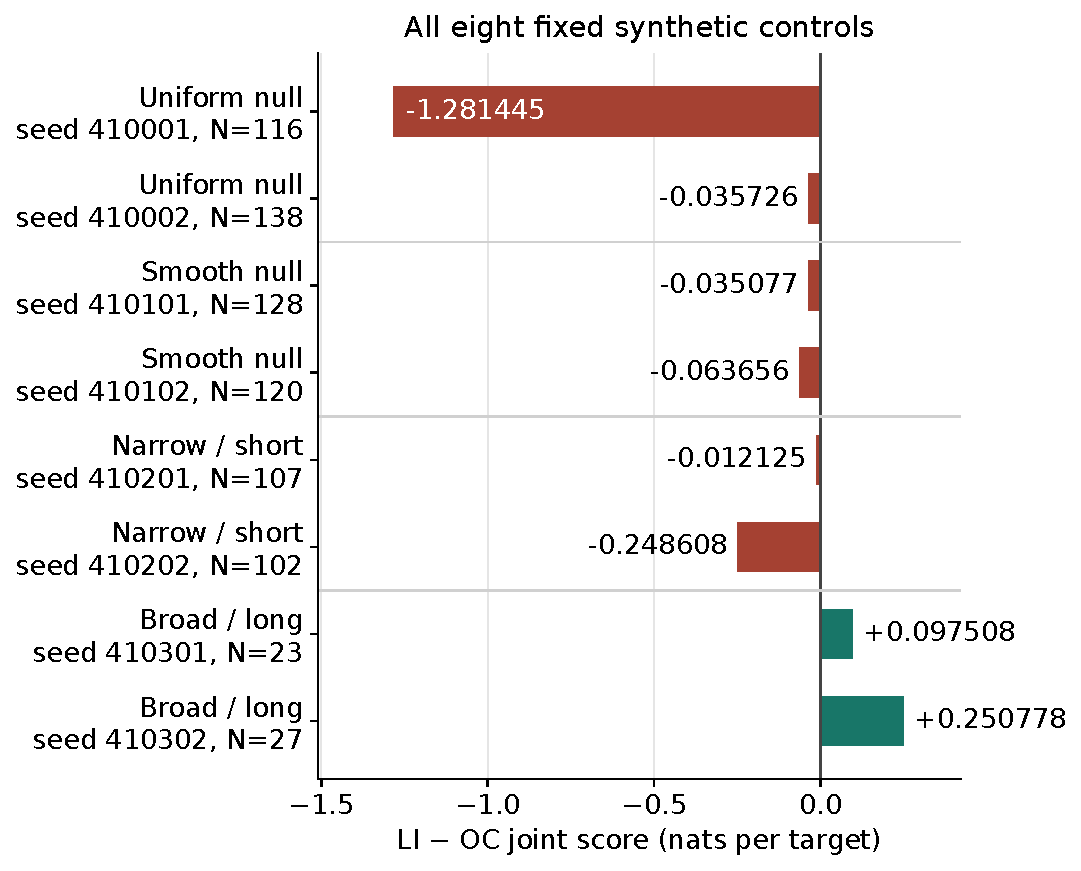
\includegraphics[width=\linewidth,height=.78\textheight,keepaspectratio]{spatial_addendum_v_li_fixed_controls.pdf}
\caption{All eight prescribed LI-minus-OC fixed controls. The full linear scale retains the large uniform-null loss. Every seed and test count remains labelled. Positive means LI scored better; the rows are fixed examples, not estimated success probabilities.}\end{figure}
\clearpage



\subsection{What the controls do and do not show}

Both broad/long wins show that the registered procedure can improve held-out score on those two fixed examples. Both narrow/short losses show why the observed zero-strength result cannot be read as a reliable absence test. A true positive term in the generating law need not improve this finite-sample fitted procedure's held-out score. Conversely, an active fitted term or better score would not identify a physical mechanism.

Two seeds per regime cannot estimate false-positive rate, power, parameter coverage or general recovery probability. Six losses do not prove absence of inhibition in the generating laws, and two wins do not establish reliable detection. Narrow/short failure does not locate a physical resolution threshold. The recorded-coordinate law has no admitted empirical location-error distribution; the engineering lower bound $\ell$ = 5 km is a model/search constraint, not a measurement-accuracy assertion.

\section{Identifiability and consolidated scientific implications}

At $\eta$ = 0 the likelihood does not depend on $\ell$ or $\psi$. Thus zero-strength selection does not estimate a zero range or duration: it removes those coordinates from the law. The null also lies at the boundary of a constrained parameter space. Exact nesting alone justifies neither ordinary Wilks inference nor a universal half-chi-square reference. No significance, p-value or event-iid confidence interval is reported.

The finite multistart procedure is part of the estimand. Negative held-out differences are possible even for nested model families because training-defined selection and finite samples do not guarantee held-out superiority. The complete retained candidates and near-optimal checks reduce particular numerical concerns; they do not certify a global optimum or prove that no positive-inhibition state could ever perform better. The conclusion must stay about the registered procedure and this history.

Together with Chapter~\ref{ch:external}, the programme supports a qualified predictive conclusion. Continuous offspring geography improves location relative to the declared cell-lift procedure in the examined regional comparisons. Omori's timing advantage is conditional and reverses in Japan. OC and its zero-inhibition LI extension remain below EP jointly in California; EP also wins in Japan. OC and EP both show fixed-state conditional discrepancies in Section~\ref{sec:s05-completed}; prospective calibration remains separate. California score gains are heterogeneous and concentrated in a single eligible scored sequence period while retaining positive contextual totals over the complete complement.

The new LI result adds a negative extension finding: no selected active inhibition and no predictive gain over matched OC in the observed windows. It does not overturn the earlier location ablation, reverse the serious-benchmark deficit, resolve calibration, recover physical labels or prove absence of a physical mechanism. The eight controls reinforce the need to distinguish procedural sensitivity from a physical absence claim.

All archives had been inspected and revised. Chronological test windows are related through overlapping training history and earthquake dependence, and the same California targets recur across studies. No pristine confirmation, broad independent sequence replication or causal conclusion follows. The prospective New Zealand programme remains readiness only; future capture, issuance and scoring are separate from these historical results. This chapter provides no issued-forecast outcomes, scheduling activation or publication decision.

\section{Numerical completion is a separate validation result}

The historical initial completed roster contains 19 fit procedures: paired OC/LI fits for eight synthetic datasets plus three observed LI fits. It accounts for 152 prescribed starts and 30 floors, giving 182 final slots. Seventeen historical CPU fits were preserved; the two remaining observed fits completed with the admitted GPU provider. Nineteen score jobs replayed all candidates and finite feasible solver returns. These are computation denominators, not 19 empirical replications.

The 42 validation jobs comprise 38 procedure-phase audits, three paired sealed-reference jobs covering six comparator states, and a separate censored-attempt preservation audit. The earlier interrupted LI pool remains excluded from the final eligible pool and preserved separately; its partial success did not select the final computational epoch. Recovery changed execution machinery within the frozen scientific law and roster. No observed event was removed and no synthetic seed was replaced.

All 19 training-defined near-optimal spreads are below 0.01 nats per target; the largest is 0.00053761640079144. The exact aggregate checker passed 369 checks, with independent saved-output review and arithmetic reconstruction. Gradient statuses are fully accounted for. These checks support custody and numerical consistency under tested states, not universal gradient representability, scientific replication, physical scale recovery or global optimization.

\section{Evidence and reading guide}

The accepted scientific report is the source for observed results, all controls and completion counts. The computational provenance report preserves execution/recovery boundaries. The current evidence index routes the unchanged aggregate, source pins, complete claim bindings and field semantics. The evidence catalogue, readable protocol subset and review guide supply the exact source identities, full scientific contract and inspection order.

Claim families LI-OBSERVED, LI-CONTROLS and LI-VALIDATION separate the scientific result, fixed examples and numerical evidence. CA-BENCHMARK and CA-CALIBRATION supply the earlier comparator/calibration context; OPS-READINESS supplies the separate future-operations boundary. Current figure arithmetic is reproduced from accepted scalars; underlying fits, simulations and audits remain source-reported. Raw records, event caches and fitted vectors remain outside the review bundle. External scientific inspection is pending.

\section{Expanded fixed-backbone controls and magnitude-scaled inhibition}

\label{sec:s04-expanded}

The original S04 completed campaign expands the fixed-seed control matrix and evaluates magnitude-scaled immigrant-only and total-intensity inhibition (LI+). The earlier eight examples above remain historical results under their original numerical procedure. The expanded results below use the same declared generating regimes and shared fixed background/excitation inputs; they are not full joint nuisance refits.

The original S04 positive-control histories are generated by the original unit-mark, immigrant-only LI law. Magnitude-scaled LI+ and total-intensity attenuation are alternative fitted procedures on those same histories, not their matched generating models. Their contrast therefore measures performance under that specified generator; it does not establish relative power when magnitude-scaled or total-intensity inhibition generates the data.

The original S04 expanded roster contains 80 distinct histories, 20 in each regime, with five paired procedure/gate combinations and 400 score rows. The stress field is
\[
G_+(t,z)=\sum_{t_j<t}\exp\{\gamma Q_j-(t-t_j)/\psi\}
 \left(1+\|z-z_j\|^2/\ell^2\right)^{-2},\qquad
\gamma=\tfrac34\log 10.
\]
Here $Q_j$ is excess magnitude, so the reference excess is zero. Original LI uses the same field with unit magnitude weights. This bounded design retains a common shadow radius; it does not fit a magnitude-dependent rupture radius. With the shared fixed backbone written $B+nH$, the two LI+ intensities are
\[
 \lambda_{\rm imm}=B e^{-\eta G_+}+nH,
 \qquad \lambda_{\rm total}=(B+nH)e^{-\eta G_+}.
\]
The gate retains an active fit only when its training log-likelihood improvement exceeds $\tfrac32\log N_{\rm train}$.

The BIC-style gate is a training-only complexity penalty, not a Davies-calibrated test or a nominal-size guarantee. The gate can select the exact uninhibited floor. A held-out win and an active training fit are distinct outcomes. No seed was redrawn and no negative score was removed.

\begingroup\footnotesize\setlength{\tabcolsep}{3pt}

\begin{longtable}{@{}llrrrrr@{}}

\toprule Regime & Procedure & $N$ & Mean gain & MC SE & Median & Wins \\

\midrule\endfirsthead

\toprule Regime & Procedure & $N$ & Mean gain & MC SE & Median & Wins \\

\midrule\endhead

\bottomrule\endlastfoot

Uniform null & LI & 20 & -2.9299 & 0.9259 & -1.6435 & 3 \\

Uniform null & LI+ immigrant gated & 20 & 0.0000 & 0.0000 & 0.0000 & 0 \\

Uniform null & LI+ immigrant & 20 & -2.9514 & 1.3451 & -0.3835 & 4 \\

Uniform null & LI+ total gated & 20 & 0.0000 & 0.0000 & 0.0000 & 0 \\

Uniform null & LI+ total & 20 & -74.6499 & 42.9783 & -2.2181 & 1 \\

Smooth null & LI & 20 & -3.4230 & 1.3263 & -2.2716 & 4 \\

Smooth null & LI+ immigrant gated & 20 & 0.0000 & 0.0000 & 0.0000 & 0 \\

Smooth null & LI+ immigrant & 20 & -3.6408 & 1.5156 & -1.9787 & 4 \\

Smooth null & LI+ total gated & 20 & 0.0000 & 0.0000 & 0.0000 & 0 \\

Smooth null & LI+ total & 20 & -448.5272 & 445.0217 & -0.0604 & 3 \\

Narrow/short & LI & 20 & -3.8713 & 1.3147 & -2.3528 & 3 \\

Narrow/short & LI+ immigrant gated & 20 & 0.0000 & 0.0000 & 0.0000 & 0 \\

Narrow/short & LI+ immigrant & 20 & -3.4720 & 1.6063 & -1.1309 & 4 \\

Narrow/short & LI+ total gated & 20 & 0.0000 & 0.0000 & 0.0000 & 0 \\

Narrow/short & LI+ total & 20 & -129.3344 & 103.6071 & -0.6334 & 6 \\

Broad/long & LI & 20 & 33.8922 & 1.2083 & 33.4049 & 20 \\

Broad/long & LI+ immigrant gated & 20 & 28.3296 & 1.6682 & 26.6651 & 20 \\

Broad/long & LI+ immigrant & 20 & 28.3296 & 1.6682 & 26.6651 & 20 \\

Broad/long & LI+ total gated & 20 & -5.4013 & 13.7572 & 3.9231 & 10 \\

Broad/long & LI+ total & 20 & -5.3446 & 13.7585 & 4.4063 & 14 \\

\end{longtable}\endgroup

Mean and median gains are total held-out log-score differences from the shared uninhibited baseline; MC SE is the sample standard deviation divided by the square root of the number of independent seeded datasets within each regime. It is a descriptive finite-sample summary, not a calibrated confidence interval. The unbounded magnitude transforms and large retained losses do not by themselves establish finite score variance or a Gaussian approximation. The broad/long regime supports improved mean performance for original LI and immigrant-only LI+. Total-intensity attenuation has a negative mean even there, despite a positive median. The large negative means in other regimes are retained rather than trimmed.

In original S04, gating selects the uninhibited floor throughout both null regimes, but also throughout the narrow/short positive regime. This demonstrates the sensitivity--overfitting tradeoff of this procedure on these controls; it does not establish nominal Type I error or general detection power.

The original S04 completed matrix combines accepted first-pass results with quadrature refinement and same-history finer-grid refits. Training-only selection preserves the prescribed starts, bounds and exact uninhibited floor. Finer-grid validation checks retained candidates, score decomposition and forecast spread. Independent compiled CPU replays cover predeclared anchors; the remaining cases have per-case numerical checks and sampled-audit coverage, not individual independent replay. All aggregate tables and their source identities are retained in the evidence bundle.

These results extend the synthetic evidence only. They do not replace the observed California comparison, for which the completed observed LI+ evaluation is reported in Section~\ref{sec:s04-observed-completed} below.

\begin{figure}[p]\centering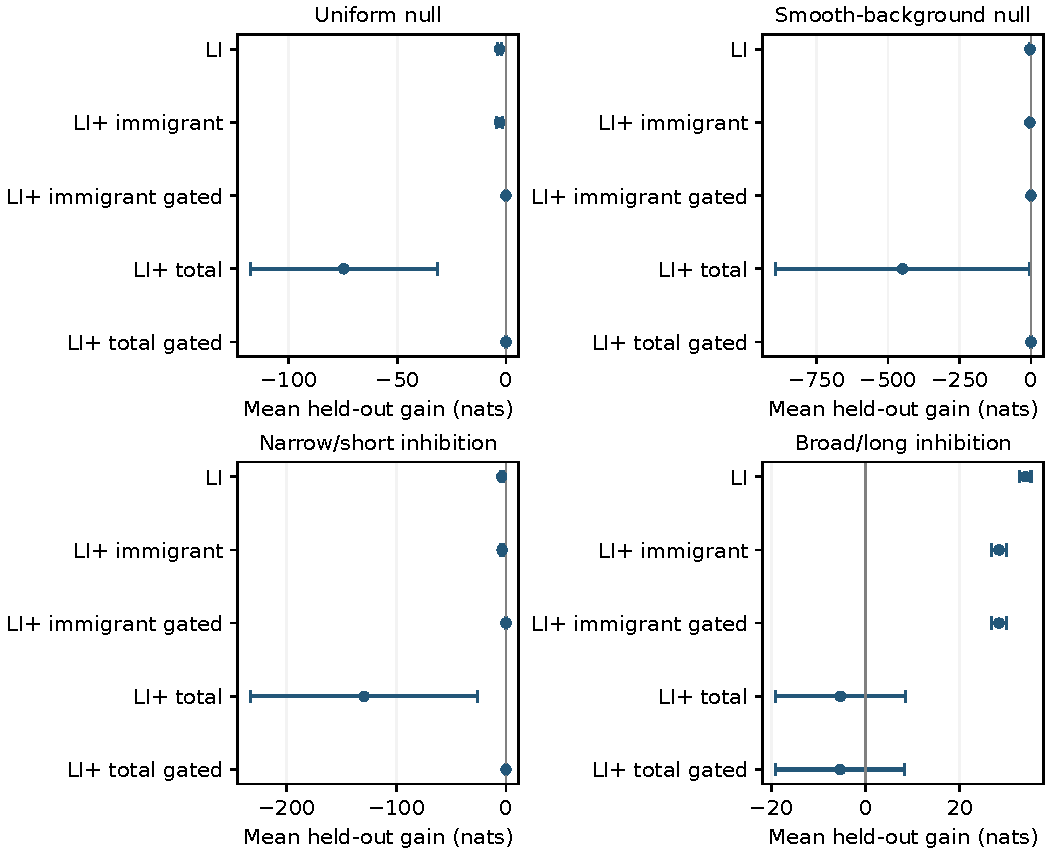
\includegraphics[width=\linewidth]{s04_unitmark_mean_gains.pdf}
\caption{Original S04 unit-mark fixed-backbone controls. Points show mean held-out gain and bars show the descriptive sample standard deviation divided by the square root of the row denominator, labelled MC SE in the table. These bars are not calibrated confidence intervals. Panels retain their full linear ranges, including large losses; horizontal scales differ. Each plotted summary uses the full corresponding row denominator in the preceding table. The zero line is the shared uninhibited comparator.}\end{figure}


\subsection{Matched magnitude-scaled generators (S04B)}

\label{sec:s04b-matched}

S04B is a separate matched-generator extension, not a replacement for the unit-mark S04 controls above. Magnitude-scaled immigrant-only and total-intensity laws each generate narrow/short and broad/long positive controls. Only accepted events enter the strictly prior stress field and spawn descendants. Immigrant-only generation thins immigrant proposals; total-intensity generation also thins offspring proposals.

The completed extension contains 80 independent seeded histories and 400 paired procedure scores. Every regime--procedure row has 20 histories. The five procedures share each history and are not independent replications. The original null histories remain valid at zero inhibition; they are not regenerated or added to this positive-control denominator.

Generation uses the smooth background and the same day-based split as the original controls: warmup $[0, 30)$, training $[30, 395)$ and test $[395, 760)$, with horizon $760$ days. For each generating law, narrow/short inhibition has $(\eta,\ell,\psi)=(0.5,5\ {\rm km},1/24\ {\rm day})$ and broad/long inhibition has $(2.0,50\ {\rm km},30\ {\rm days})$. The magnitude scaling and the two intensity definitions are those displayed above. Seeds are predeclared and retained without replacement: immigrant narrow/short $410401$ through $410420$, immigrant broad/long $410501$ through $410520$, total narrow/short $410601$ through $410620$, and total broad/long $410701$ through $410720$. Training uses all $8$ prescribed starts plus the exact uninhibited floor at quadrature order $16$; every retained finite state is checked at order $32$ on training and test windows. The first seed in each regime is the predeclared independent CPU anchor. These settings and source identities are retained in the bundled frozen-method projection and protocol.

All fits hold the shared background and excitation backbone fixed. Training-only selection and the complexity gate retain the exact uninhibited floor. Full saved-row arithmetic and numerical gates are audited; independent CPU objective and gradient replays cover 48 predeclared phase--model contexts from the anchor histories, rather than every history.

Under immigrant: narrow/short generation, the matched raw procedure has a negative mean gain and a negative median; its gated version has a negative mean. Under immigrant: broad/long generation, the matched raw procedure has a positive mean gain and a positive median; its gated version has a positive mean. Under total: narrow/short generation, the matched raw procedure has a negative mean gain and a negative median; its gated version has a positive mean. Under total: broad/long generation, the matched raw procedure has a positive mean gain and a positive median; its gated version has a positive mean. Both matched raw procedures lose on average in their narrow/short settings. The positive gated mean under narrow/short total generation comes from a single winning active history and otherwise exact-floor ties; it does not demonstrate reliable recovery. Under narrow/short immigrant generation, the matched gate instead retains a single active loss and otherwise floor ties. In both broad/long generating settings, matched raw and gated procedures win on every history in this declared bank. These outcomes remain conditional on the fixed nuisance backbone and chosen regimes.

Mean and median gains below are total held-out log-score differences per simulated history, not per earthquake. MC SE is the within-regime sample standard deviation divided by the square root of the history denominator. It is descriptive: these heavy-tailed marked laws do not supply an automatic finite-variance or Gaussian guarantee. Wilson intervals describe bounded held-out-win indicators under the declared seeded simulation design; they are not intervals for the mean gain or calibrated detection power. A positive held-out gain, an active fit and an identified physical mechanism are different statements.

\begingroup\footnotesize\setlength{\tabcolsep}{3pt}

\begin{longtable}{@{}lrrrrrrr@{}}

\caption{S04B: Immigrant: narrow/short. Wins are strict positive gains; interval endpoints are probabilities.}\label{tab:s04b-4}\\

\toprule Procedure & $N$ & Mean & MC SE & Median & Wins & Wilson 95\% & Active \\

\midrule\endfirsthead

\toprule Procedure & $N$ & Mean & MC SE & Median & Wins & Wilson 95\% & Active \\

\midrule\endhead

\bottomrule\endlastfoot

LI & 20 & -3.9493 & 1.2142 & -2.7555 & 2 & [0.028, 0.301] & 19 \\

LI+ immigrant & 20 & -4.5674 & 1.6218 & -2.0582 & 5 & [0.112, 0.469] & 20 \\

LI+ immigrant gated & 20 & -1.3440 & 1.3440 & 0.0000 & 0 & [0.000, 0.161] & 1 \\

LI+ total & 20 & -21.5766 & 9.8329 & -3.1228 & 4 & [0.081, 0.416] & 19 \\

LI+ total gated & 20 & -1.0043 & 1.0043 & 0.0000 & 0 & [0.000, 0.161] & 1 \\

\end{longtable}\endgroup

\begingroup\footnotesize\setlength{\tabcolsep}{3pt}

\begin{longtable}{@{}lrrrrrrr@{}}

\caption{S04B: Immigrant: broad/long. Wins are strict positive gains; interval endpoints are probabilities.}\label{tab:s04b-5}\\

\toprule Procedure & $N$ & Mean & MC SE & Median & Wins & Wilson 95\% & Active \\

\midrule\endfirsthead

\toprule Procedure & $N$ & Mean & MC SE & Median & Wins & Wilson 95\% & Active \\

\midrule\endhead

\bottomrule\endlastfoot

LI & 20 & 44.3122 & 1.4559 & 43.3861 & 20 & [0.839, 1.000] & 20 \\

LI+ immigrant & 20 & 48.3868 & 0.9599 & 47.7879 & 20 & [0.839, 1.000] & 20 \\

LI+ immigrant gated & 20 & 48.3868 & 0.9599 & 47.7879 & 20 & [0.839, 1.000] & 20 \\

LI+ total & 20 & 19.4993 & 7.2001 & 35.3378 & 15 & [0.531, 0.888] & 19 \\

LI+ total gated & 20 & 19.3802 & 7.2159 & 35.3378 & 14 & [0.481, 0.855] & 18 \\

\end{longtable}\endgroup

\begingroup\footnotesize\setlength{\tabcolsep}{3pt}

\begin{longtable}{@{}lrrrrrrr@{}}

\caption{S04B: Total: narrow/short. Wins are strict positive gains; interval endpoints are probabilities.}\label{tab:s04b-6}\\

\toprule Procedure & $N$ & Mean & MC SE & Median & Wins & Wilson 95\% & Active \\

\midrule\endfirsthead

\toprule Procedure & $N$ & Mean & MC SE & Median & Wins & Wilson 95\% & Active \\

\midrule\endhead

\bottomrule\endlastfoot

LI & 20 & -1.7818 & 0.6357 & -0.9047 & 5 & [0.112, 0.469] & 20 \\

LI+ immigrant & 20 & -3.2420 & 1.2527 & -0.5371 & 7 & [0.181, 0.567] & 20 \\

LI+ immigrant gated & 20 & 0.0000 & 0.0000 & 0.0000 & 0 & [0.000, 0.161] & 0 \\

LI+ total & 20 & -14.5947 & 7.8248 & -0.1064 & 10 & [0.299, 0.701] & 20 \\

LI+ total gated & 20 & 0.0686 & 0.0686 & 0.0000 & 1 & [0.009, 0.236] & 1 \\

\end{longtable}\endgroup

\clearpage

\begingroup\footnotesize\setlength{\tabcolsep}{3pt}

\begin{longtable}{@{}lrrrrrrr@{}}

\caption{S04B: Total: broad/long. Wins are strict positive gains; interval endpoints are probabilities.}\label{tab:s04b-7}\\

\toprule Procedure & $N$ & Mean & MC SE & Median & Wins & Wilson 95\% & Active \\

\midrule\endfirsthead

\toprule Procedure & $N$ & Mean & MC SE & Median & Wins & Wilson 95\% & Active \\

\midrule\endhead

\bottomrule\endlastfoot

LI & 20 & 42.5503 & 1.7274 & 44.8818 & 20 & [0.839, 1.000] & 20 \\

LI+ immigrant & 20 & 49.2902 & 1.3502 & 48.5828 & 20 & [0.839, 1.000] & 20 \\

LI+ immigrant gated & 20 & 49.2902 & 1.3502 & 48.5828 & 20 & [0.839, 1.000] & 20 \\

LI+ total & 20 & 53.2332 & 2.1250 & 51.2906 & 20 & [0.839, 1.000] & 20 \\

LI+ total gated & 20 & 53.2332 & 2.1250 & 51.2906 & 20 & [0.839, 1.000] & 20 \\

\end{longtable}\endgroup

Active counts record off-floor selection ($\hat\eta > 0$), including the effect of the training-only gate. The bundled public audit exports score contrasts and off-floor indicators rather than empirical distributions of selected $(\hat\eta,\hat\ell,\hat\psi)$: S04B evaluates held-out predictive log-score gain rather than parameter recovery. An active fit can still overfit or adjust shared coordinates without recovering the generating $(\eta,\ell,\psi)$. Zero gains remain ties, not wins. No negative gain is trimmed and no seed is substituted. The completed matched generation resolves the prior generating-law gap for these bounded settings; it does not resolve joint nuisance estimation, nominal test size, general recovery or prospective observational evidence.

\begin{figure}[p]\centering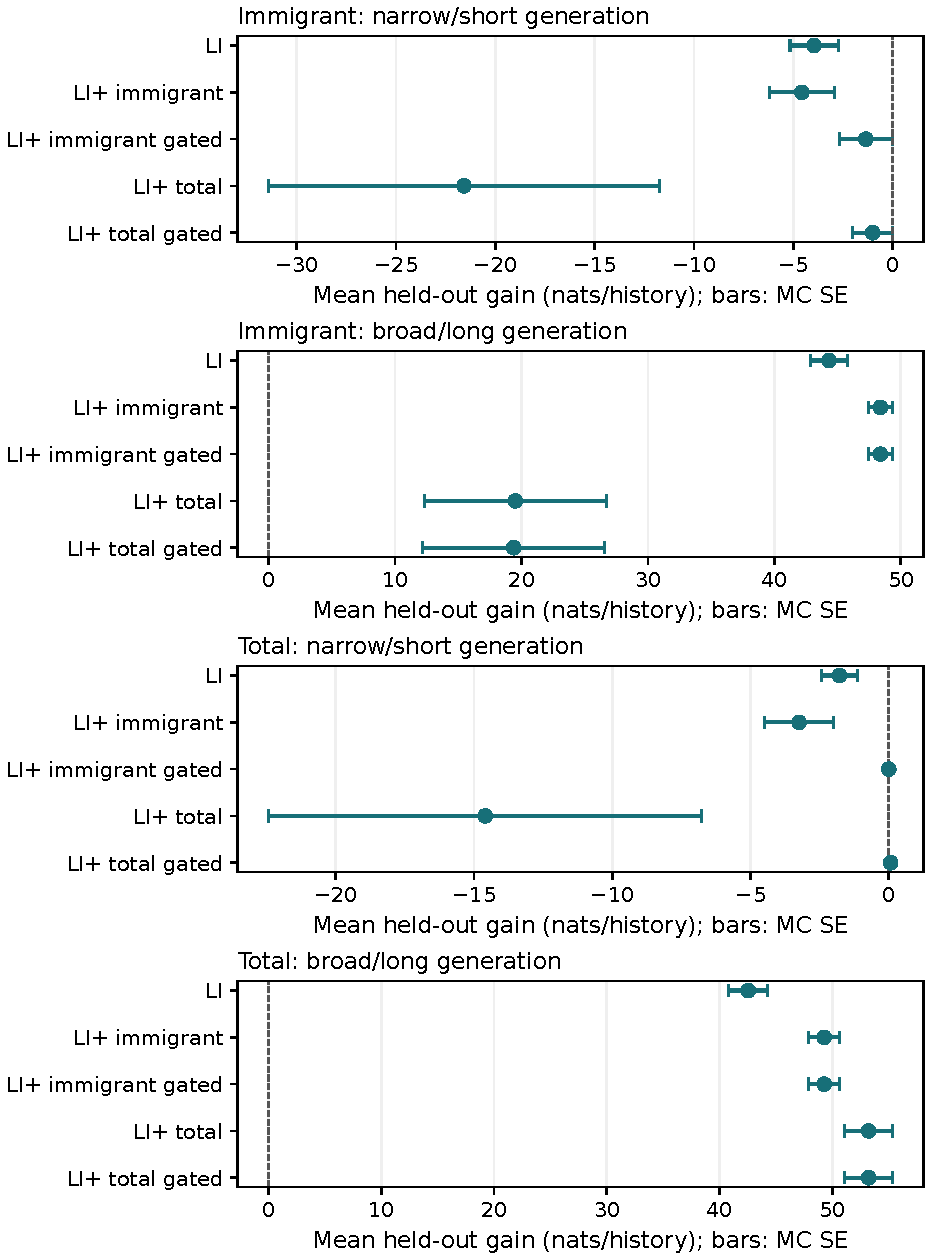
\includegraphics[width=\linewidth]{s04_expanded_mean_gains.pdf}

\caption{S04B matched-generator controls. Each panel keeps its own full linear range. Points show row means; bars show descriptive MC SE, not calibrated confidence intervals. Each procedure uses the same complete history denominator within its generating regime. The dashed zero line denotes the uninhibited floor; regimes are not pooled.}\label{fig:s04b-matched}\end{figure}


\section{Observed California fixed-backbone inhibition}

\label{sec:s04-observed-completed}

The observed comparison uses the same three California folds and 315 targets. Background and excitation nuisance inputs are fixed and shared between each candidate and its exact uninhibited floor. The common mark term cancels from each held-out joint gain, reported as floor NLL minus selected NLL.

Original LI is retained unpenalized. Magnitude-scaled LI+ is evaluated with immigrant-only and total-intensity attenuation, each with raw training selection and with the declared training-only BIC-style gate. A gate may select the exact floor. A negative held-out gain is retained, while an unresolved numerical result remains unknown rather than being assigned zero.

Table~\ref{tab:s04-observed} reports the three active empirical contrasts. Table~\ref{tab:s04-observed-boundary} partitions the twelve gate-selected or nested rows whose training solution is $\hat\eta=0$: for these cells the held-out joint contrast is identically $0.0000$ by algebraic nesting, not an independent empirical test of zero attenuation. Presenting the twelve zero rows as separate powered comparisons would overstate the evidence.

\begin{table}[htbp]\centering\caption{Active held-out joint gains (nats) relative to the shared uninhibited floor. All three rows select positive total-intensity attenuation in training and lose held-out joint score. Displayed values are empirical contrasts, not algebraic returns. Paired block intervals for raw total-intensity attenuation are reported in Section~\ref{sec:li-score-uncertainty}.}\label{tab:s04-observed}

\begin{tabular}{llllrll}\toprule Fold & Model & Gate & Status & Gain & Win & Active\\\midrule

0 & LI+ total & raw & resolved & -0.2245 & no & yes \\

1 & LI+ total & raw & resolved & -1.9529 & no & yes \\

2 & LI+ total & raw & resolved & -0.2093 & no & yes \\

\bottomrule\end{tabular}\end{table}

\begin{table}[htbp]\centering\caption{Boundary-selected rows partitioned from the active contrasts. Each displayed $0.0000$ is the exact algebraic forecast of the nested $\hat\eta=0$ floor, not an estimate of a zero physical effect. The twelve cells are three folds of four floor-selected procedures and must not be counted as twelve independent empirical test contrasts.}\label{tab:s04-observed-boundary}

\begin{tabular}{llllr}\toprule Fold & Model & Gate & Status & Algebraic gain\\\midrule

0 & LI & raw & floor-selected & 0.0000 \\

0 & LI+ immigrant & raw & floor-selected & 0.0000 \\

0 & LI+ immigrant & BIC & floor-selected & 0.0000 \\

0 & LI+ total & BIC & floor-selected & 0.0000 \\

1 & LI & raw & floor-selected & 0.0000 \\

1 & LI+ immigrant & raw & floor-selected & 0.0000 \\

1 & LI+ immigrant & BIC & floor-selected & 0.0000 \\

1 & LI+ total & BIC & floor-selected & 0.0000 \\

2 & LI & raw & floor-selected & 0.0000 \\

2 & LI+ immigrant & raw & floor-selected & 0.0000 \\

2 & LI+ immigrant & BIC & floor-selected & 0.0000 \\

2 & LI+ total & BIC & floor-selected & 0.0000 \\

\bottomrule\end{tabular}\end{table}

The BIC-style gate is a complexity penalty, not a Davies-calibrated test or a guarantee of nominal size. A training-active fit, a selected floor and a held-out win are distinct outcomes. These observed folds have been inspected retrospectively.

\begin{figure}[p]\centering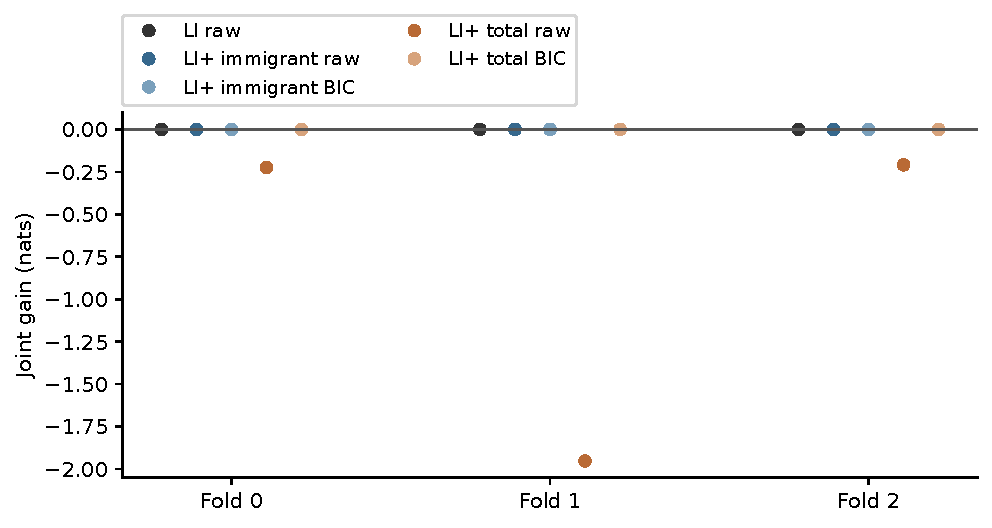
\includegraphics[width=\textwidth]{s04_observed_joint_gains.pdf}\caption{Held-out joint gains on the fixed three-fold population.}\end{figure}

\begin{center}\begin{tabular}{lrr}\toprule Fold & Training targets & Planned held-out targets\\\midrule

0 & 851 & 79 \\

1 & 930 & 167 \\

2 & 1097 & 69 \\

\bottomrule\end{tabular}\end{center}

All original LI and magnitude-scaled immigrant-only fits select their exact uninhibited floor. Raw total-intensity inhibition is active but loses held-out joint score in each fold. Its BIC-gated version selects the floor in every fold. These outcomes do not establish a predictive benefit from the revised inhibition mechanisms on this fixed observed population.

